\begin{tikzpicture}
  \begin{scope}[scale = 2]
    \def\slingringsmonn{.2}
    \def\majorradius{1}
    \def\minorradius{.5}
    \def\miniradius{.1}
    \def\verticaldilation{.5}
    \draw[thick, -latex] (0, {-\verticaldilation*.5*pi-\slingringsmonn})--(0, {\verticaldilation*.5*pi + \slingringsmonn}) node[left]{$\eta$};
    \draw[thick, -latex] ({-(.5*pi+\slingringsmonn)}, 0)--({(.5*pi + \slingringsmonn)}, 0) node[below right]{$\theta$};
    \draw[thick] ({-.5*pi}, .1)--({-.5*pi}, -.1) node[below]{$-\sfrac{\pi}{2}$};
    \draw[thick] ({.5*pi}, .1)--({.5*pi}, -.1) node[below]{$\sfrac{\pi}{2}$};
    \draw[thick] (.1, {-\verticaldilation*(.5*pi)})--(-.1, {-\verticaldilation*(.5*pi)}) node[left]{$-\sfrac{\pi}{2}$};
    \draw[thick] (.1, {\verticaldilation*(.5*pi)})--(-.1, {\verticaldilation*(.5*pi)}) node[left]{$\sfrac{\pi}{2}$};
    \def\smallvalue{.05}
    \draw[domain = {-.5*pi+\smallvalue}:{.5*pi-\smallvalue}, smooth, thick] plot (\x, {\verticaldilation*rad(atan(\majorradius*tan(\x r)/\minorradius))});
    \draw[domain = {-.5*pi+\smallvalue}:{.5*pi-\smallvalue}, smooth, dashed, thick] plot (\x, {\verticaldilation*rad(atan(\majorradius*tan(\x r)/\miniradius))});
  \end{scope}
\end{tikzpicture}
